\documentclass{standalone}
\usepackage{tikz}
\usetikzlibrary{patterns, positioning}


\begin{document}
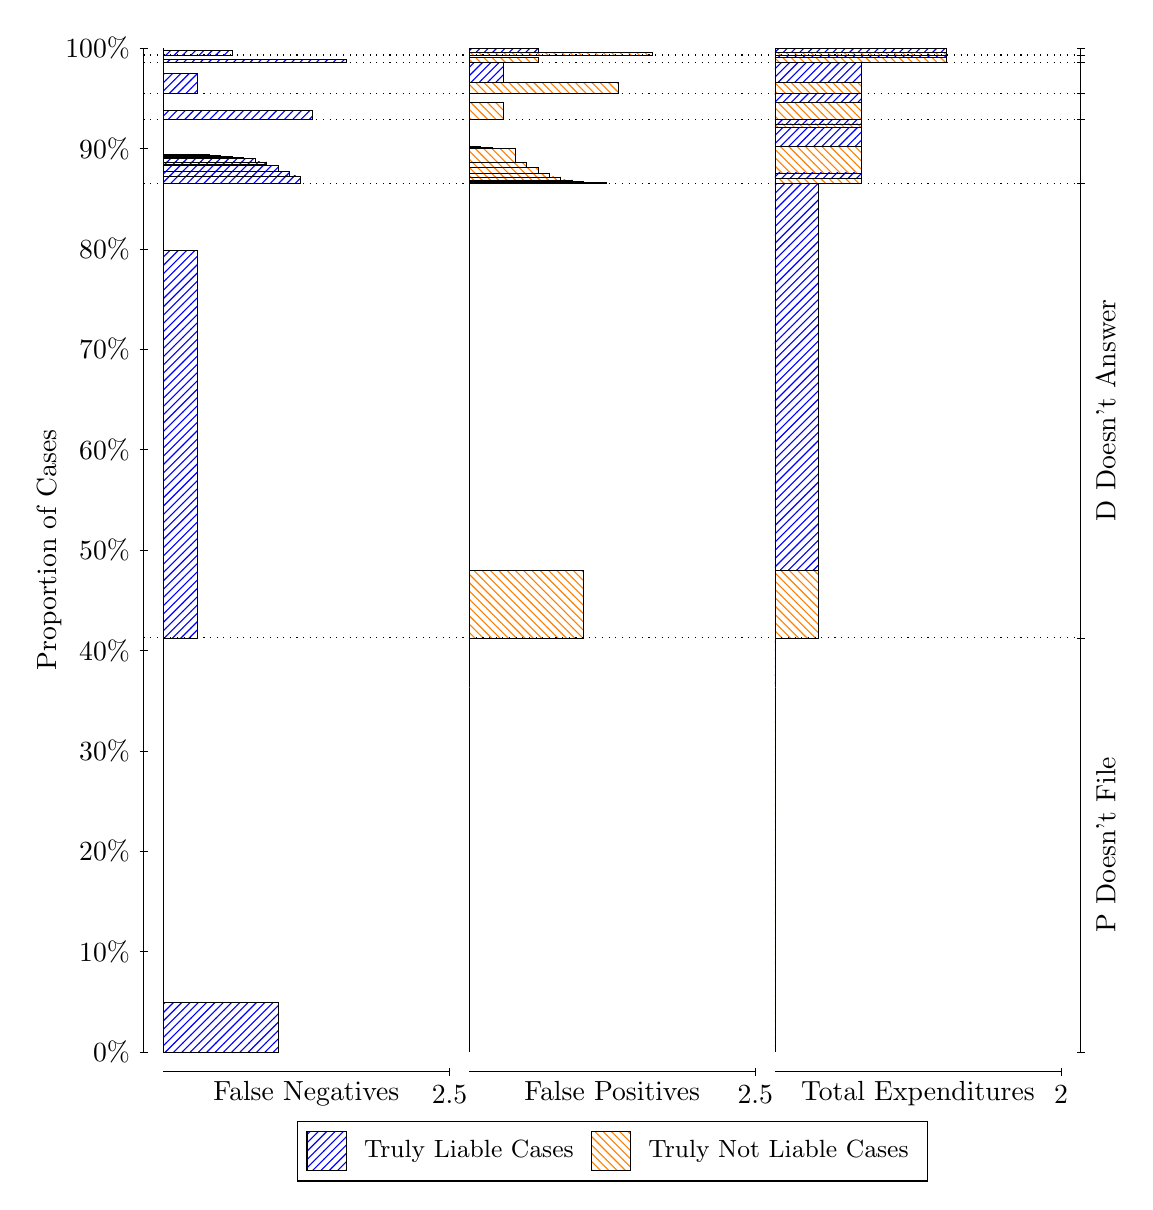
\begin{tikzpicture}
\draw[black, very thin] (1.5,1.75) -- (1.5,14.5);
\node[rotate=90, text=black, anchor=center] at (0.3, 8.125) {Proportion of Cases};
\draw[black, very thin] (1.45,1.75) -- (1.55,1.75);
\node[text=black, anchor=east] at (1.45, 1.75) {0\%};
\draw[black, very thin] (1.45,3.025) -- (1.55,3.025);
\node[text=black, anchor=east] at (1.45, 3.025) {10\%};
\draw[black, very thin] (1.45,4.3) -- (1.55,4.3);
\node[text=black, anchor=east] at (1.45, 4.3) {20\%};
\draw[black, very thin] (1.45,5.575) -- (1.55,5.575);
\node[text=black, anchor=east] at (1.45, 5.575) {30\%};
\draw[black, very thin] (1.45,6.85) -- (1.55,6.85);
\node[text=black, anchor=east] at (1.45, 6.85) {40\%};
\draw[black, very thin] (1.45,8.125) -- (1.55,8.125);
\node[text=black, anchor=east] at (1.45, 8.125) {50\%};
\draw[black, very thin] (1.45,9.4) -- (1.55,9.4);
\node[text=black, anchor=east] at (1.45, 9.4) {60\%};
\draw[black, very thin] (1.45,10.675) -- (1.55,10.675);
\node[text=black, anchor=east] at (1.45, 10.675) {70\%};
\draw[black, very thin] (1.45,11.95) -- (1.55,11.95);
\node[text=black, anchor=east] at (1.45, 11.95) {80\%};
\draw[black, very thin] (1.45,13.225) -- (1.55,13.225);
\node[text=black, anchor=east] at (1.45, 13.225) {90\%};
\draw[black, very thin] (1.45,14.5) -- (1.55,14.5);
\node[text=black, anchor=east] at (1.45, 14.5) {100\%};

\draw[black, very thin] (13.4,1.75) -- (13.4,14.5);
\draw[black, very thin] (13.35,1.75) -- (13.45,1.75);
\node[anchor=west] at (13.35, 1.75) {};
\draw[black, very thin] (13.35,7.01) -- (13.45,7.01);
\node[anchor=west] at (13.35, 7.01) {};
\draw[black, very thin] (13.35,12.785) -- (13.45,12.785);
\node[anchor=west] at (13.35, 12.785) {};
\draw[black, very thin] (13.35,13.592) -- (13.45,13.592);
\node[anchor=west] at (13.35, 13.592) {};
\draw[black, very thin] (13.35,13.924) -- (13.45,13.924);
\node[anchor=west] at (13.35, 13.924) {};
\draw[black, very thin] (13.35,14.317) -- (13.45,14.317);
\node[anchor=west] at (13.35, 14.317) {};
\draw[black, very thin] (13.35,14.411) -- (13.45,14.411);
\node[anchor=west] at (13.35, 14.411) {};
\draw[black, very thin] (13.35,14.5) -- (13.45,14.5);
\node[anchor=west] at (13.35, 14.5) {};

\draw[black, very thin, pattern color=blue, pattern=north east lines] (1.75,1.75) rectangle (3.2033,2.3828);
\draw[black, very thin, pattern color=orange, pattern=north west lines] (1.75,2.3828) rectangle (1.75,7.01);
\draw[black, very thin, pattern color=blue, pattern=north east lines] (1.75,7.01) rectangle (2.186,11.926);
\draw[black, very thin, pattern color=orange, pattern=north west lines] (1.75,11.926) rectangle (1.75,12.785);
\draw[black, very thin, pattern color=blue, pattern=north east lines] (1.75,12.785) rectangle (3.494,12.877);
\draw[black, very thin, pattern color=blue, pattern=north east lines] (1.75,12.877) rectangle (3.3487,12.932);
\draw[black, very thin, pattern color=blue, pattern=north east lines] (1.75,12.932) rectangle (3.2033,13.011);
\draw[black, very thin, pattern color=blue, pattern=north east lines] (1.75,13.011) rectangle (3.058,13.027);
\draw[black, very thin, pattern color=blue, pattern=north east lines] (1.75,13.027) rectangle (3.058,13.054);
\draw[black, very thin, pattern color=blue, pattern=north east lines] (1.75,13.054) rectangle (2.9127,13.094);
\draw[black, very thin, pattern color=blue, pattern=north east lines] (1.75,13.094) rectangle (2.7673,13.107);
\draw[black, very thin, pattern color=blue, pattern=north east lines] (1.75,13.107) rectangle (2.622,13.126);
\draw[black, very thin, pattern color=blue, pattern=north east lines] (1.75,13.126) rectangle (2.4767,13.136);
\draw[black, very thin, pattern color=blue, pattern=north east lines] (1.75,13.136) rectangle (2.3313,13.151);
\draw[black, very thin, pattern color=orange, pattern=north west lines] (1.75,13.151) rectangle (1.75,13.592);
\draw[black, very thin, pattern color=blue, pattern=north east lines] (1.75,13.592) rectangle (3.6393,13.71);
\draw[black, very thin, pattern color=orange, pattern=north west lines] (1.75,13.71) rectangle (1.75,13.924);
\draw[black, very thin, pattern color=blue, pattern=north east lines] (1.75,13.924) rectangle (2.186,14.177);
\draw[black, very thin, pattern color=orange, pattern=north west lines] (1.75,14.177) rectangle (1.75,14.317);
\draw[black, very thin, pattern color=blue, pattern=north east lines] (1.75,14.317) rectangle (4.0753,14.351);
\draw[black, very thin, pattern color=orange, pattern=north west lines] (1.75,14.351) rectangle (1.75,14.411);
\draw[black, very thin, pattern color=blue, pattern=north east lines] (1.75,14.411) rectangle (2.622,14.467);
\draw[black, very thin, pattern color=orange, pattern=north west lines] (1.75,14.467) rectangle (1.75,14.5);
\draw[black, very thin, pattern color=orange, pattern=north west lines] (5.6333,1.75) rectangle (5.6333,6.3773);
\draw[black, very thin, pattern color=blue, pattern=north east lines] (5.6333,6.3773) rectangle (5.6333,7.01);
\draw[black, very thin, pattern color=orange, pattern=north west lines] (5.6333,7.01) rectangle (7.0867,7.8691);
\draw[black, very thin, pattern color=blue, pattern=north east lines] (5.6333,7.8691) rectangle (5.6333,12.785);
\draw[black, very thin, pattern color=orange, pattern=north west lines] (5.6333,12.785) rectangle (7.3773,12.791);
\draw[black, very thin, pattern color=orange, pattern=north west lines] (5.6333,12.791) rectangle (7.232,12.798);
\draw[black, very thin, pattern color=orange, pattern=north west lines] (5.6333,12.798) rectangle (7.0867,12.811);
\draw[black, very thin, pattern color=orange, pattern=north west lines] (5.6333,12.811) rectangle (6.9413,12.824);
\draw[black, very thin, pattern color=orange, pattern=north west lines] (5.6333,12.824) rectangle (6.796,12.863);
\draw[black, very thin, pattern color=orange, pattern=north west lines] (5.6333,12.863) rectangle (6.6507,12.906);
\draw[black, very thin, pattern color=orange, pattern=north west lines] (5.6333,12.906) rectangle (6.5053,12.989);
\draw[black, very thin, pattern color=orange, pattern=north west lines] (5.6333,12.989) rectangle (6.36,13.052);
\draw[black, very thin, pattern color=orange, pattern=north west lines] (5.6333,13.052) rectangle (6.2147,13.226);
\draw[black, very thin, pattern color=blue, pattern=north east lines] (5.6333,13.226) rectangle (5.924,13.241);
\draw[black, very thin, pattern color=blue, pattern=north east lines] (5.6333,13.241) rectangle (5.7787,13.25);
\draw[black, very thin, pattern color=blue, pattern=north east lines] (5.6333,13.25) rectangle (5.6333,13.592);
\draw[black, very thin, pattern color=orange, pattern=north west lines] (5.6333,13.592) rectangle (6.0693,13.806);
\draw[black, very thin, pattern color=blue, pattern=north east lines] (5.6333,13.806) rectangle (5.6333,13.924);
\draw[black, very thin, pattern color=orange, pattern=north west lines] (5.6333,13.924) rectangle (7.5227,14.065);
\draw[black, very thin, pattern color=blue, pattern=north east lines] (5.6333,14.065) rectangle (6.0693,14.317);
\draw[black, very thin, pattern color=orange, pattern=north west lines] (5.6333,14.317) rectangle (6.5053,14.377);
\draw[black, very thin, pattern color=blue, pattern=north east lines] (5.6333,14.377) rectangle (5.6333,14.411);
\draw[black, very thin, pattern color=orange, pattern=north west lines] (5.6333,14.411) rectangle (7.9587,14.444);
\draw[black, very thin, pattern color=blue, pattern=north east lines] (5.6333,14.444) rectangle (6.5053,14.5);
\draw[black, very thin, pattern color=orange, pattern=north west lines] (9.5167,1.75) rectangle (9.5167,6.3773);
\draw[black, very thin, pattern color=blue, pattern=north east lines] (9.5167,6.3773) rectangle (9.5167,7.01);
\draw[black, very thin, pattern color=orange, pattern=north west lines] (9.5167,7.01) rectangle (10.062,7.8691);
\draw[black, very thin, pattern color=blue, pattern=north east lines] (9.5167,7.8691) rectangle (10.062,12.785);
\draw[black, very thin, pattern color=orange, pattern=north west lines] (9.5167,12.785) rectangle (10.607,12.845);
\draw[black, very thin, pattern color=blue, pattern=north east lines] (9.5167,12.845) rectangle (10.607,12.914);
\draw[black, very thin, pattern color=orange, pattern=north west lines] (9.5167,12.914) rectangle (10.607,13.249);
\draw[black, very thin, pattern color=blue, pattern=north east lines] (9.5167,13.249) rectangle (10.607,13.492);
\draw[black, very thin, pattern color=orange, pattern=north west lines] (9.5167,13.492) rectangle (10.607,13.537);
\draw[black, very thin, pattern color=blue, pattern=north east lines] (9.5167,13.537) rectangle (10.607,13.592);
\draw[black, very thin, pattern color=orange, pattern=north west lines] (9.5167,13.592) rectangle (10.607,13.806);
\draw[black, very thin, pattern color=blue, pattern=north east lines] (9.5167,13.806) rectangle (10.607,13.924);
\draw[black, very thin, pattern color=orange, pattern=north west lines] (9.5167,13.924) rectangle (10.607,14.065);
\draw[black, very thin, pattern color=blue, pattern=north east lines] (9.5167,14.065) rectangle (10.607,14.317);
\draw[black, very thin, pattern color=orange, pattern=north west lines] (9.5167,14.317) rectangle (11.697,14.377);
\draw[black, very thin, pattern color=blue, pattern=north east lines] (9.5167,14.377) rectangle (11.697,14.411);
\draw[black, very thin, pattern color=orange, pattern=north west lines] (9.5167,14.411) rectangle (11.697,14.444);
\draw[black, very thin, pattern color=blue, pattern=north east lines] (9.5167,14.444) rectangle (11.697,14.5);
\draw[black, dotted] (1.5,7.01) -- (13.4,7.01);
\draw[black, dotted] (1.5,12.785) -- (13.4,12.785);
\draw[black, dotted] (1.5,13.592) -- (13.4,13.592);
\draw[black, dotted] (1.5,13.924) -- (13.4,13.924);
\draw[black, dotted] (1.5,14.317) -- (13.4,14.317);
\draw[black, dotted] (1.5,14.411) -- (13.4,14.411);
\draw[black, very thin] (1.75,1.5) -- (5.3833,1.5);
\node[text=black, anchor=north] at (3.5667, 1.5) {False Negatives};
\draw[black, very thin] (5.3833,1.45) -- (5.3833,1.55);
\node[text=black, anchor=north] at (5.3833, 1.45) {2.5};

\draw[black, very thin] (5.6333,1.5) -- (9.2667,1.5);
\node[text=black, anchor=north] at (7.45, 1.5) {False Positives};
\draw[black, very thin] (9.2667,1.45) -- (9.2667,1.55);
\node[text=black, anchor=north] at (9.2667, 1.45) {2.5};

\draw[black, very thin] (9.5167,1.5) -- (13.15,1.5);
\node[text=black, anchor=north] at (11.333, 1.5) {Total Expenditures};
\draw[black, very thin] (13.15,1.45) -- (13.15,1.55);
\node[text=black, anchor=north] at (13.15, 1.45) {2};

\node[text=black, centered, rotate=90] at (13.72, 4.38) {P Doesn't File};
\node[text=black, centered, rotate=90] at (13.72, 9.8975) {D Doesn't Answer};






\draw (7.449999999999999,1.5) node[draw=none] (baseCoordinate) {};
\begin{scope}[align=center]
        \matrix[scale=0.5, draw=black, below=0.5cm of baseCoordinate, nodes={draw}, column sep=0.1cm]{
            \node[rectangle, draw, minimum width=0.5cm, minimum height=0.5cm, pattern color=blue, pattern=north east lines] {}; &
            \node[draw=none, font=\small, text=black] (B) {Truly Liable Cases}; &
            \node[rectangle, draw, minimum width=0.5cm, minimum height=0.5cm, pattern color=orange, pattern=north west lines] {}; &
            \node[draw=none, font=\small, text=black] (B) {Truly Not Liable Cases}; \\
            };
\end{scope}

\end{tikzpicture}
\end{document}